% Options for packages loaded elsewhere
\PassOptionsToPackage{unicode}{hyperref}
\PassOptionsToPackage{hyphens}{url}
\PassOptionsToPackage{dvipsnames,svgnames*,x11names*}{xcolor}
%
\documentclass[
  ignorenonframetext,
]{beamer}
\usepackage{pgfpages}
\setbeamertemplate{caption}[numbered]
\setbeamertemplate{caption label separator}{: }
\setbeamercolor{caption name}{fg=normal text.fg}
\beamertemplatenavigationsymbolsempty
% Prevent slide breaks in the middle of a paragraph
\widowpenalties 1 10000
\raggedbottom
\setbeamertemplate{part page}{
  \centering
  \begin{beamercolorbox}[sep=16pt,center]{part title}
    \usebeamerfont{part title}\insertpart\par
  \end{beamercolorbox}
}
\setbeamertemplate{section page}{
  \centering
  \begin{beamercolorbox}[sep=12pt,center]{part title}
    \usebeamerfont{section title}\insertsection\par
  \end{beamercolorbox}
}
\setbeamertemplate{subsection page}{
  \centering
  \begin{beamercolorbox}[sep=8pt,center]{part title}
    \usebeamerfont{subsection title}\insertsubsection\par
  \end{beamercolorbox}
}
\AtBeginPart{
  \frame{\partpage}
}
\AtBeginSection{
  \ifbibliography
  \else
    \frame{\sectionpage}
  \fi
}
\AtBeginSubsection{
  \frame{\subsectionpage}
}
\usepackage{lmodern}
\usepackage{amssymb,amsmath}
\usepackage{ifxetex,ifluatex}
\ifnum 0\ifxetex 1\fi\ifluatex 1\fi=0 % if pdftex
  \usepackage[T1]{fontenc}
  \usepackage[utf8]{inputenc}
  \usepackage{textcomp} % provide euro and other symbols
\else % if luatex or xetex
  \usepackage{unicode-math}
  \defaultfontfeatures{Scale=MatchLowercase}
  \defaultfontfeatures[\rmfamily]{Ligatures=TeX,Scale=1}
\fi
% Use upquote if available, for straight quotes in verbatim environments
\IfFileExists{upquote.sty}{\usepackage{upquote}}{}
\IfFileExists{microtype.sty}{% use microtype if available
  \usepackage[]{microtype}
  \UseMicrotypeSet[protrusion]{basicmath} % disable protrusion for tt fonts
}{}
\makeatletter
\@ifundefined{KOMAClassName}{% if non-KOMA class
  \IfFileExists{parskip.sty}{%
    \usepackage{parskip}
  }{% else
    \setlength{\parindent}{0pt}
    \setlength{\parskip}{6pt plus 2pt minus 1pt}}
}{% if KOMA class
  \KOMAoptions{parskip=half}}
\makeatother
\usepackage{xcolor}
\IfFileExists{xurl.sty}{\usepackage{xurl}}{} % add URL line breaks if available
\IfFileExists{bookmark.sty}{\usepackage{bookmark}}{\usepackage{hyperref}}
\hypersetup{
  pdftitle={Regression and ANOVA},
  pdfauthor={Zack Treisman},
  colorlinks=true,
  linkcolor=Maroon,
  filecolor=Maroon,
  citecolor=blue,
  urlcolor=Blue,
  pdfcreator={LaTeX via pandoc}}
\urlstyle{same} % disable monospaced font for URLs
\newif\ifbibliography
\usepackage{color}
\usepackage{fancyvrb}
\newcommand{\VerbBar}{|}
\newcommand{\VERB}{\Verb[commandchars=\\\{\}]}
\DefineVerbatimEnvironment{Highlighting}{Verbatim}{commandchars=\\\{\}}
% Add ',fontsize=\small' for more characters per line
\usepackage{framed}
\definecolor{shadecolor}{RGB}{248,248,248}
\newenvironment{Shaded}{\begin{snugshade}}{\end{snugshade}}
\newcommand{\AlertTok}[1]{\textcolor[rgb]{0.94,0.16,0.16}{#1}}
\newcommand{\AnnotationTok}[1]{\textcolor[rgb]{0.56,0.35,0.01}{\textbf{\textit{#1}}}}
\newcommand{\AttributeTok}[1]{\textcolor[rgb]{0.77,0.63,0.00}{#1}}
\newcommand{\BaseNTok}[1]{\textcolor[rgb]{0.00,0.00,0.81}{#1}}
\newcommand{\BuiltInTok}[1]{#1}
\newcommand{\CharTok}[1]{\textcolor[rgb]{0.31,0.60,0.02}{#1}}
\newcommand{\CommentTok}[1]{\textcolor[rgb]{0.56,0.35,0.01}{\textit{#1}}}
\newcommand{\CommentVarTok}[1]{\textcolor[rgb]{0.56,0.35,0.01}{\textbf{\textit{#1}}}}
\newcommand{\ConstantTok}[1]{\textcolor[rgb]{0.00,0.00,0.00}{#1}}
\newcommand{\ControlFlowTok}[1]{\textcolor[rgb]{0.13,0.29,0.53}{\textbf{#1}}}
\newcommand{\DataTypeTok}[1]{\textcolor[rgb]{0.13,0.29,0.53}{#1}}
\newcommand{\DecValTok}[1]{\textcolor[rgb]{0.00,0.00,0.81}{#1}}
\newcommand{\DocumentationTok}[1]{\textcolor[rgb]{0.56,0.35,0.01}{\textbf{\textit{#1}}}}
\newcommand{\ErrorTok}[1]{\textcolor[rgb]{0.64,0.00,0.00}{\textbf{#1}}}
\newcommand{\ExtensionTok}[1]{#1}
\newcommand{\FloatTok}[1]{\textcolor[rgb]{0.00,0.00,0.81}{#1}}
\newcommand{\FunctionTok}[1]{\textcolor[rgb]{0.00,0.00,0.00}{#1}}
\newcommand{\ImportTok}[1]{#1}
\newcommand{\InformationTok}[1]{\textcolor[rgb]{0.56,0.35,0.01}{\textbf{\textit{#1}}}}
\newcommand{\KeywordTok}[1]{\textcolor[rgb]{0.13,0.29,0.53}{\textbf{#1}}}
\newcommand{\NormalTok}[1]{#1}
\newcommand{\OperatorTok}[1]{\textcolor[rgb]{0.81,0.36,0.00}{\textbf{#1}}}
\newcommand{\OtherTok}[1]{\textcolor[rgb]{0.56,0.35,0.01}{#1}}
\newcommand{\PreprocessorTok}[1]{\textcolor[rgb]{0.56,0.35,0.01}{\textit{#1}}}
\newcommand{\RegionMarkerTok}[1]{#1}
\newcommand{\SpecialCharTok}[1]{\textcolor[rgb]{0.00,0.00,0.00}{#1}}
\newcommand{\SpecialStringTok}[1]{\textcolor[rgb]{0.31,0.60,0.02}{#1}}
\newcommand{\StringTok}[1]{\textcolor[rgb]{0.31,0.60,0.02}{#1}}
\newcommand{\VariableTok}[1]{\textcolor[rgb]{0.00,0.00,0.00}{#1}}
\newcommand{\VerbatimStringTok}[1]{\textcolor[rgb]{0.31,0.60,0.02}{#1}}
\newcommand{\WarningTok}[1]{\textcolor[rgb]{0.56,0.35,0.01}{\textbf{\textit{#1}}}}
\usepackage{graphicx,grffile}
\makeatletter
\def\maxwidth{\ifdim\Gin@nat@width>\linewidth\linewidth\else\Gin@nat@width\fi}
\def\maxheight{\ifdim\Gin@nat@height>\textheight\textheight\else\Gin@nat@height\fi}
\makeatother
% Scale images if necessary, so that they will not overflow the page
% margins by default, and it is still possible to overwrite the defaults
% using explicit options in \includegraphics[width, height, ...]{}
\setkeys{Gin}{width=\maxwidth,height=\maxheight,keepaspectratio}
% Set default figure placement to htbp
\makeatletter
\def\fps@figure{htbp}
\makeatother
\setlength{\emergencystretch}{3em} % prevent overfull lines
\providecommand{\tightlist}{%
  \setlength{\itemsep}{0pt}\setlength{\parskip}{0pt}}
\setcounter{secnumdepth}{-\maxdimen} % remove section numbering

\pgfdeclareimage[width=3.5cm]{mcslogo}{../western_logo_hor_MCS_3C_pos.pdf}
\pgfdeclareimage[width=1cm]{ccbysa}{../ccbysa88x31.png}
\titlegraphic{\href{http://creativecommons.org/licenses/by-sa/4.0/}{\pgfuseimage{ccbysa}}
\hfill
\href{https://western.edu/program/mathematics/}{\pgfuseimage{mcslogo}}}
%\usecolortheme{wcu}
%\institute{Western Colorado University}
%\setbeamertemplate{navigation symbols}{}

\title{Regression and ANOVA}
\author{Zack Treisman}
\date{Spring 2021}

\begin{document}
\frame{\titlepage}

\begin{frame}{Philosophy}
\protect\hypertarget{philosophy}{}

\textbf{Regression} generally refers to a family of techniques where a
model \(\hat{y}=f(x)\) is fit to data \((x_i, y_i)\) such that the
\textbf{mean squared error} \[
MSE=\frac{1}{n}\sum_{i=1}^n(y_i-\hat{y})^2
\] is as small as possible given \emph{a priori} assumptions on the form
of \(f(x)\), such as being a linear function \(f(x)=\beta_0+\beta_1 x\).

Regression is the starting point for linear regression, ANOVA and
several other classical techniques.

\end{frame}

\begin{frame}{Linear Regression}
\protect\hypertarget{linear-regression}{}

Linear regression posits a relationship between two numerical random
variables \(X\) and \(Y\) of the form \[
Y \sim N(\beta_0+\beta_1 X, \sigma^2).
\] The parameters \(\beta_0\) (the \textbf{intercept}), \(\beta_1\) (the
\textbf{slope}) and \(\sigma^2\) (the \textbf{variance}) are estimated
from observations of \(X\) and \(Y\). Specifically, writing
\(\bar x = \sum^n_{i=1}x_i\), and \(\bar y = \sum^n_{i=1}y_i\) for the
sample means and using a little calculus, \[
\hat \beta_1 = \frac{\sum^n_{i=1}(x_i-\bar x)(y_i-\bar y)}{\sum^n_{i=1}(x_i-\bar x)^2}, \quad
\hat \beta_0 = \bar y - \hat\beta_1\bar x.
\] The variance of the \textbf{residuals} \(y_i-\hat{y}\) gives the
estimate of \(\sigma^2\).

\end{frame}

\begin{frame}[fragile]{The data linear regression expects}
\protect\hypertarget{the-data-linear-regression-expects}{}

Estimates from these formulas are expected to be accurate when \(X\) is
uniformly distributed and \(Y\) is normally distributed about a linear
function of \(X\). \scriptsize

\begin{Shaded}
\begin{Highlighting}[]
\KeywordTok{set.seed}\NormalTok{(}\DecValTok{5}\NormalTok{)}
\NormalTok{x <-}\StringTok{ }\KeywordTok{runif}\NormalTok{(}\DecValTok{100}\NormalTok{)}
\NormalTok{y <-}\StringTok{ }\KeywordTok{rnorm}\NormalTok{(}\DecValTok{100}\NormalTok{, }\DataTypeTok{mean =} \DecValTok{1} \OperatorTok{+}\StringTok{ }\DecValTok{2}\OperatorTok{*}\NormalTok{x, }\DataTypeTok{sd =} \FloatTok{0.5}\NormalTok{)}
\KeywordTok{plot}\NormalTok{(y}\OperatorTok{~}\NormalTok{x)}
\KeywordTok{abline}\NormalTok{(}\DecValTok{1}\NormalTok{,}\DecValTok{2}\NormalTok{, }\DataTypeTok{col=}\StringTok{"blue"}\NormalTok{)}
\end{Highlighting}
\end{Shaded}

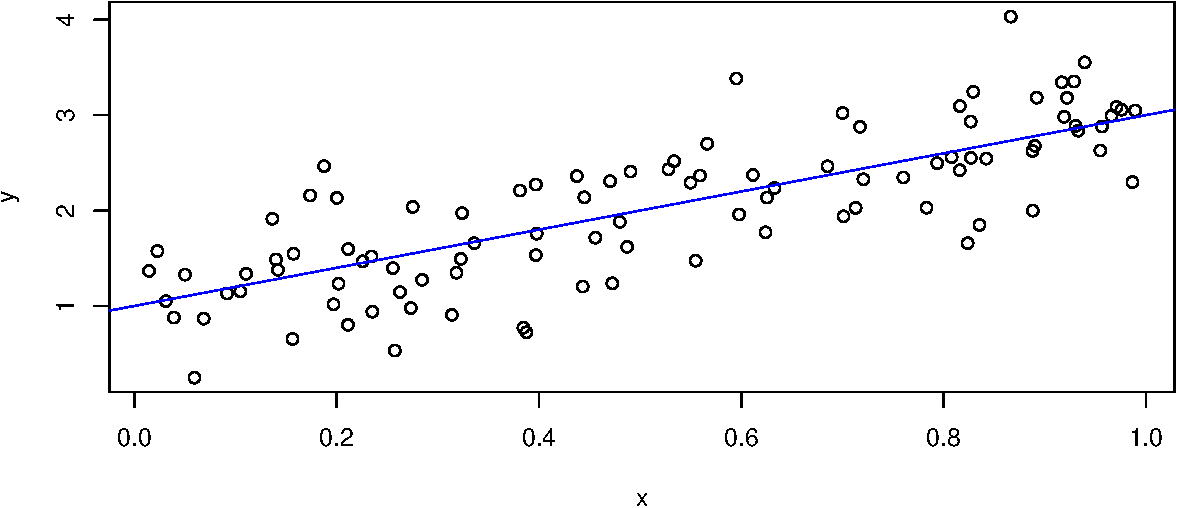
\includegraphics{Regression_and_ANOVA_files/figure-beamer/unnamed-chunk-2-1.pdf}

\end{frame}

\begin{frame}[fragile]{The \texttt{lm} function in R}
\protect\hypertarget{the-lm-function-in-r}{}

\scriptsize

\begin{Shaded}
\begin{Highlighting}[]
\NormalTok{lm1 <-}\StringTok{ }\KeywordTok{lm}\NormalTok{(y}\OperatorTok{~}\NormalTok{x)}
\NormalTok{lm1}\OperatorTok{$}\NormalTok{coefficients}
\end{Highlighting}
\end{Shaded}

\begin{verbatim}
## (Intercept)           x 
##   0.9515095   2.0764806
\end{verbatim}

\begin{Shaded}
\begin{Highlighting}[]
\KeywordTok{plot}\NormalTok{(y}\OperatorTok{~}\NormalTok{x); }\KeywordTok{abline}\NormalTok{(}\DecValTok{1}\NormalTok{,}\DecValTok{2}\NormalTok{, }\DataTypeTok{col=}\StringTok{"blue"}\NormalTok{); }\KeywordTok{abline}\NormalTok{(lm1, }\DataTypeTok{col=}\StringTok{"red"}\NormalTok{)}
\end{Highlighting}
\end{Shaded}

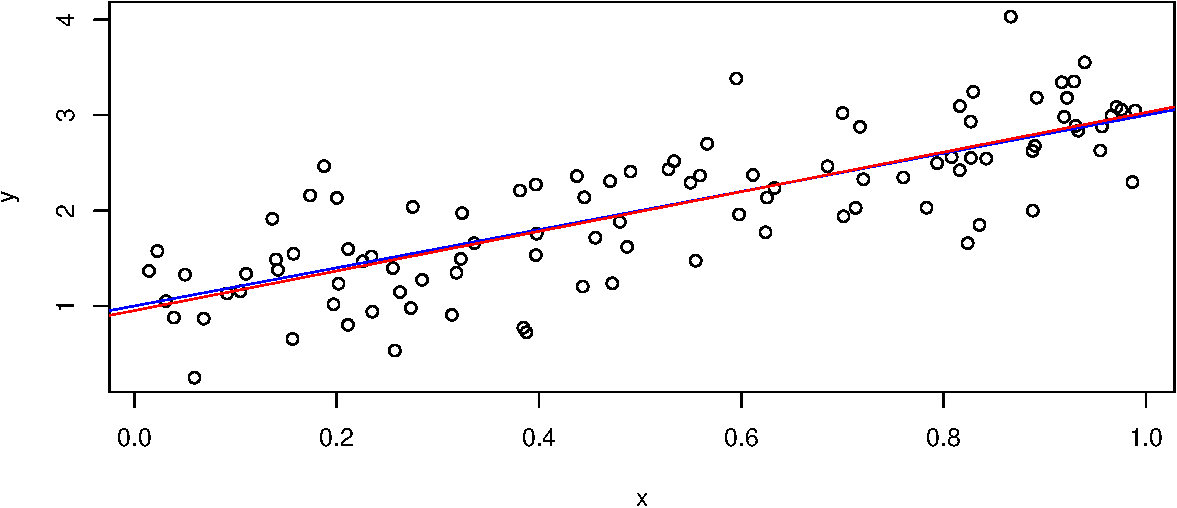
\includegraphics{Regression_and_ANOVA_files/figure-beamer/unnamed-chunk-3-1.pdf}

\end{frame}

\begin{frame}[fragile]{Evaluating a linear model}
\protect\hypertarget{evaluating-a-linear-model}{}

\scriptsize

\begin{Shaded}
\begin{Highlighting}[]
\KeywordTok{summary}\NormalTok{(lm1)}
\end{Highlighting}
\end{Shaded}

\begin{verbatim}
## 
## Call:
## lm(formula = y ~ x)
## 
## Residuals:
##      Min       1Q   Median       3Q      Max 
## -1.03231 -0.26608 -0.01308  0.35581  1.28230 
## 
## Coefficients:
##             Estimate Std. Error t value Pr(>|t|)    
## (Intercept)  0.95151    0.09657   9.853 2.52e-16 ***
## x            2.07648    0.16104  12.895  < 2e-16 ***
## ---
## Signif. codes:  0 '***' 0.001 '**' 0.01 '*' 0.05 '.' 0.1 ' ' 1
## 
## Residual standard error: 0.4853 on 98 degrees of freedom
## Multiple R-squared:  0.6292, Adjusted R-squared:  0.6254 
## F-statistic: 166.3 on 1 and 98 DF,  p-value: < 2.2e-16
\end{verbatim}

\end{frame}

\begin{frame}[fragile]{Check residuals}
\protect\hypertarget{check-residuals}{}

Residuals appear normally distributed around 0 with a consistent
variance independent of \(X\). \scriptsize

\begin{Shaded}
\begin{Highlighting}[]
\KeywordTok{plot}\NormalTok{(lm1}\OperatorTok{$}\NormalTok{residuals}\OperatorTok{~}\NormalTok{x); }\KeywordTok{abline}\NormalTok{(}\DecValTok{0}\NormalTok{,}\DecValTok{0}\NormalTok{, }\DataTypeTok{lty=}\StringTok{"dashed"}\NormalTok{)}
\end{Highlighting}
\end{Shaded}

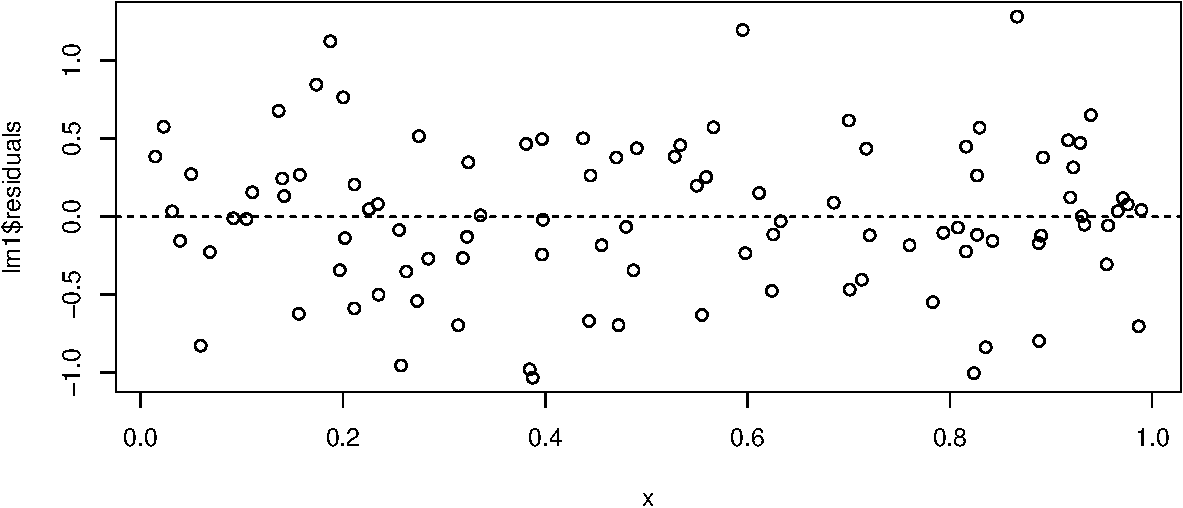
\includegraphics{Regression_and_ANOVA_files/figure-beamer/unnamed-chunk-5-1.pdf}

\normalsize

We'll discuss various ways to check homogeneity of variance. There's no
one correct way to do it.

\end{frame}

\begin{frame}{Overall accuracy of the model}
\protect\hypertarget{overall-accuracy-of-the-model}{}

\(R^2\) measures how much the variance in \(Y\) is described by the
model.

\[
R^2 = 1 - \frac{\sigma_\text{residuals}^2}{\sigma_y^2} = 1 - \frac{\sum_{i=1}^n(y_i-\hat y)^2}{\sum_{i=1}^n(y_i-\bar y)^2}
\]
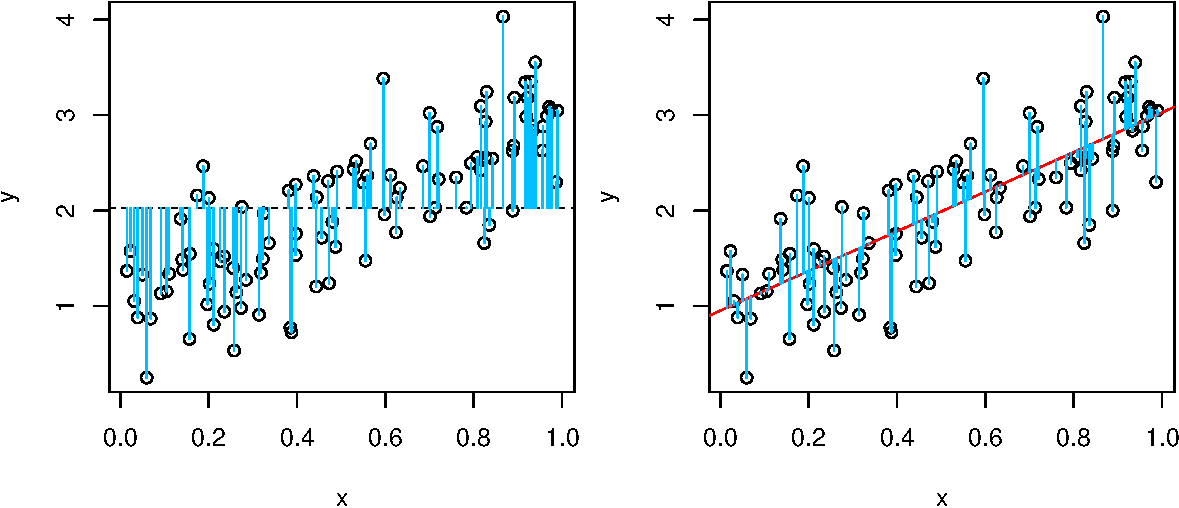
\includegraphics{Regression_and_ANOVA_files/figure-beamer/unnamed-chunk-6-1.pdf}
We'll talk about Adjusted \(R^2\) and the \(F\)-statistic shortly.

\end{frame}

\begin{frame}{Accuracy of the coefficient estimates}
\protect\hypertarget{accuracy-of-the-coefficient-estimates}{}

The standard error of an estimator reflects how it varies under repeated
sampling. \[
SE(\hat\beta_1)=\sqrt{\frac{\sigma^2}{\sum_{i=1}^n(x_i-\bar x)^2}}, \quad SE(\hat\beta_0)=\sqrt{\frac{\sigma^2}{n}+\frac{\sigma^2\bar x^2}{\sum_{i=1}^n(x_i-\bar x^2)}}
\]

\begin{itemize}
\tightlist
\item
  Standard errors allow us to compute confidence intervals for these
  parameters.
\item
  For samples such as ours, there is a 95\% chance that the interval \[
  \hat\beta_1 \pm 2 \cdot SE(\hat\beta_1)
  \] contains the true value of \(\beta_1\). (Which is 2.)
\item
  In our case, the 95\% confidence interval is \[
  2.076 \pm 2 \cdot 0.161 = (1.754,2.399)
  \]
\end{itemize}

\end{frame}

\begin{frame}[fragile]{Simulate taking 5000 such samples and calculating
\(\beta_1\)}
\protect\hypertarget{simulate-taking-5000-such-samples-and-calculating-beta_1}{}

\scriptsize

\begin{Shaded}
\begin{Highlighting}[]
\NormalTok{betas <-}\StringTok{ }\KeywordTok{numeric}\NormalTok{(}\DecValTok{5000}\NormalTok{); b_captured <-}\StringTok{ }\KeywordTok{logical}\NormalTok{(}\DecValTok{5000}\NormalTok{)}
\ControlFlowTok{for}\NormalTok{(i }\ControlFlowTok{in} \DecValTok{1}\OperatorTok{:}\DecValTok{5000}\NormalTok{)\{}
\NormalTok{ x <-}\StringTok{ }\KeywordTok{runif}\NormalTok{(}\DecValTok{100}\NormalTok{); y <-}\StringTok{ }\KeywordTok{rnorm}\NormalTok{(}\DecValTok{100}\NormalTok{, }\DataTypeTok{mean =} \DecValTok{1} \OperatorTok{+}\StringTok{ }\DecValTok{2}\OperatorTok{*}\NormalTok{x, }\DataTypeTok{sd =} \FloatTok{0.5}\NormalTok{)}
\NormalTok{ lmi <-}\StringTok{ }\KeywordTok{lm}\NormalTok{(y}\OperatorTok{~}\NormalTok{x); slope <-}\StringTok{ }\KeywordTok{coef}\NormalTok{(}\KeywordTok{summary}\NormalTok{(lmi))[}\DecValTok{2}\NormalTok{,]}
\NormalTok{ betas[i] <-}\StringTok{ }\NormalTok{slope[}\DecValTok{1}\NormalTok{]}
\NormalTok{ b_captured[i] <-}\StringTok{ }\NormalTok{(}\DecValTok{2}\OperatorTok{>}\NormalTok{slope[}\DecValTok{1}\NormalTok{]}\OperatorTok{-}\FloatTok{1.96}\OperatorTok{*}\NormalTok{slope[}\DecValTok{2}\NormalTok{]) }\OperatorTok{&}\StringTok{ }\NormalTok{(}\DecValTok{2}\OperatorTok{<}\NormalTok{slope[}\DecValTok{1}\NormalTok{]}\OperatorTok{+}\FloatTok{1.96}\OperatorTok{*}\NormalTok{slope[}\DecValTok{2}\NormalTok{]) }
\NormalTok{\}}
\KeywordTok{mean}\NormalTok{(b_captured); }\KeywordTok{hist}\NormalTok{(betas)}
\end{Highlighting}
\end{Shaded}

\begin{verbatim}
## [1] 0.9526
\end{verbatim}

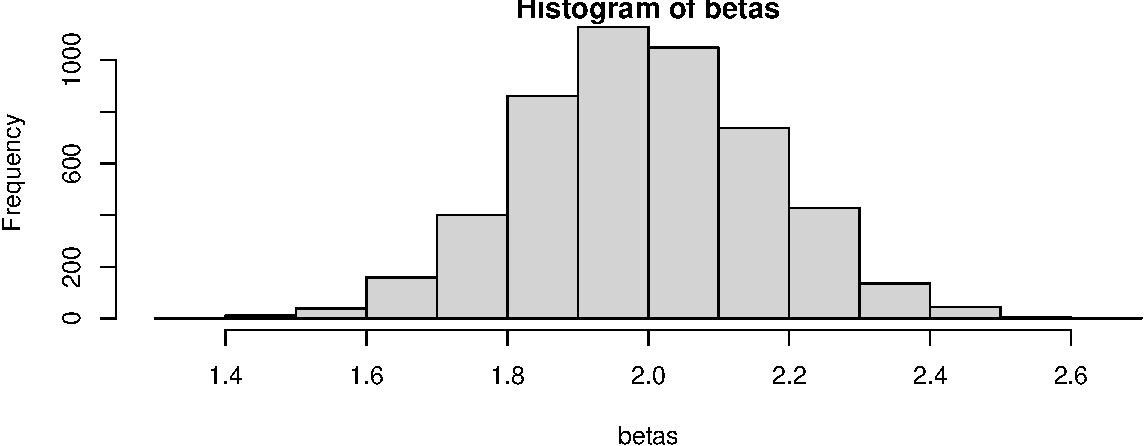
\includegraphics{Regression_and_ANOVA_files/figure-beamer/unnamed-chunk-7-1.pdf}

\end{frame}

\begin{frame}{Hypothesis testing}
\protect\hypertarget{hypothesis-testing}{}

Having the standard errors for the estimated parameters also allows us
to do hypothesis tests.

\begin{itemize}
\tightlist
\item
  Generally we are not interested in testing the intercept.
\item
  Testing the null hypothesis \[
  H_0: \beta_1=0
  \] is equivalent to testing for no relationship between \(X\) and
  \(Y\).
\item
  The \(t\) statistic for this test is \[
  t=\frac{\hat\beta_1}{SE(\hat\beta_1)}.
  \]
\item
  The null hypothesis distribution is a \(t\) distribution with \(n-2\)
  degrees of freedom.
\end{itemize}

\end{frame}

\begin{frame}{Multiple Linear Regression}
\protect\hypertarget{multiple-linear-regression}{}

The theory is similar if there are multiple predictor variables. \[
Y \sim N(\beta_0+\beta_1X_1+\beta_2X_2+\cdots+\beta_pX_p, \sigma^2)
\]

\begin{itemize}
\tightlist
\item
  The parameter \(\beta_j\) is the average effect on \(Y\) of a one unit
  increase in \(X_j\), holding all other predictors fixed.
\item
  Ideally the predictors are uncorrelated --- this is called a
  \textbf{balanced design}.

  \begin{itemize}
  \tightlist
  \item
    Each coefficient can be estimated and tested separately.
  \item
    Interpreting \(\beta_j\) as above is possible.
  \end{itemize}
\item
  Correlations among predictors cause problems:

  \begin{itemize}
  \tightlist
  \item
    The variance of all coefficients tends to increase.
  \item
    Interpretations become hazardous.
  \end{itemize}
\end{itemize}

\end{frame}

\begin{frame}{Overall accuracy of the model revisited}
\protect\hypertarget{overall-accuracy-of-the-model-revisited}{}

\(R^2\) is defined exactly as for one variable linear models.

Write \(SS_{tot}=\sum_{i=1}^n(y_i-\bar y)^2\) and
\(SS_{res}=\sum_{i=1}^n(y_i-\hat y)^2\): \[
R^2 = 1 - \frac{SS_{res}}{SS_{tot}}=\frac{SS_{tot}-SS_{res}}{SS_{tot}}.
\]

\begin{itemize}
\tightlist
\item
  An immediate problem is that even a predictor \(X_j\) that has
  \emph{nothing} to do with \(Y\) is going to give \emph{some} reduction
  in \(R^2\), because \(\hat\beta_j\) will not be \emph{exactly} zero.
\end{itemize}

\end{frame}

\begin{frame}{Two alternatives to \(R^2\)}
\protect\hypertarget{two-alternatives-to-r2}{}

\begin{itemize}
\tightlist
\item
  Adjust \(R^2\) to penalize models for having more predictors: \[
  \text{Adjusted } R^2 = 1 - \frac{SS_{res}/(n-p-1)}{SS_{tot}/(n-1)}
  \]

  \begin{itemize}
  \tightlist
  \item
    This is still (loosely) interpretable as the proportion of the
    variance in the response explained by the model.
  \item
    Nearly identical to \(R^2\) when \(n>>p\).
  \end{itemize}
\item
  Another alternative is the \(F\) statistic. \[
  F = \frac{(SS_{tot}-SS_{res})/p}{SS_{res}/(n-p-1)}
  \]

  \begin{itemize}
  \tightlist
  \item
    This will be distributed as \(F_{p,n-p-1}\) if \textbf{all} of the
    \(\beta_j\) (except possibly \(\beta_0\)) are zero, so can be used
    to test \begin{align*}
      H_0 &: \beta_1=\beta_2=\cdots=\beta_p=0 \\
      H_a &: \text{At least one of the $\beta_j$ is non-zero.}
      \end{align*}
  \end{itemize}
\end{itemize}

\end{frame}

\begin{frame}[fragile]{Multiple regression with \texttt{lm}}
\protect\hypertarget{multiple-regression-with-lm}{}

Lily data from Thomson et al. (1996). \scriptsize

\begin{Shaded}
\begin{Highlighting}[]
\NormalTok{lm2 <-}\StringTok{ }\KeywordTok{lm}\NormalTok{(flowers}\OperatorTok{~}\NormalTok{vegetative}\OperatorTok{+}\NormalTok{gopher}\OperatorTok{+}\NormalTok{moisture, }\DataTypeTok{data=}\NormalTok{Lily_sum) }\CommentTok{# data in emdbook}
\KeywordTok{summary}\NormalTok{(lm2)}
\end{Highlighting}
\end{Shaded}

\begin{verbatim}
## 
## Call:
## lm(formula = flowers ~ vegetative + gopher + moisture, data = Lily_sum)
## 
## Residuals:
##     Min      1Q  Median      3Q     Max 
## -52.512 -10.447  -2.705   7.407  79.276 
## 
## Coefficients:
##             Estimate Std. Error t value Pr(>|t|)    
## (Intercept)  24.6817     4.0273   6.129 3.40e-09 ***
## vegetative    1.0758     0.1116   9.640  < 2e-16 ***
## gopher       -2.2171     0.4127  -5.372 1.77e-07 ***
## moisture      0.1761     0.7311   0.241     0.81    
## ---
## Signif. codes:  0 '***' 0.001 '**' 0.01 '*' 0.05 '.' 0.1 ' ' 1
## 
## Residual standard error: 17.38 on 252 degrees of freedom
## Multiple R-squared:  0.4523, Adjusted R-squared:  0.4458 
## F-statistic: 69.38 on 3 and 252 DF,  p-value: < 2.2e-16
\end{verbatim}

\end{frame}

\begin{frame}[fragile]{Pairs plot of the Lily data}
\protect\hypertarget{pairs-plot-of-the-lily-data}{}

\scriptsize

\begin{Shaded}
\begin{Highlighting}[]
\KeywordTok{pairs}\NormalTok{(Lily_sum[,}\KeywordTok{c}\NormalTok{(}\StringTok{"flowers"}\NormalTok{, }\StringTok{"vegetative"}\NormalTok{, }\StringTok{"gopher"}\NormalTok{, }\StringTok{"moisture"}\NormalTok{)])}
\end{Highlighting}
\end{Shaded}

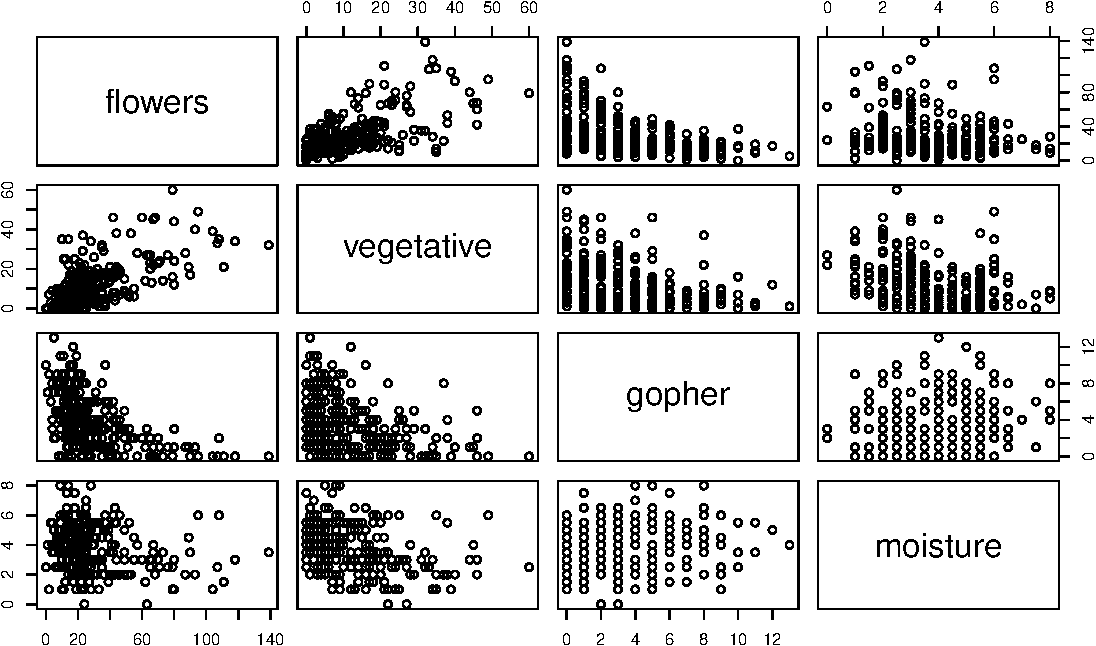
\includegraphics{Regression_and_ANOVA_files/figure-beamer/unnamed-chunk-9-1.pdf}

\end{frame}

\begin{frame}[fragile]{Confounders can have big effects}
\protect\hypertarget{confounders-can-have-big-effects}{}

The Lily data contain an additional variable. \scriptsize

\begin{Shaded}
\begin{Highlighting}[]
\NormalTok{lm3 <-}\StringTok{ }\KeywordTok{lm}\NormalTok{(flowers}\OperatorTok{~}\NormalTok{vegetative}\OperatorTok{+}\NormalTok{gopher}\OperatorTok{+}\NormalTok{moisture}\OperatorTok{+}\NormalTok{rockiness, }\DataTypeTok{data=}\NormalTok{Lily_sum)}
\KeywordTok{summary}\NormalTok{(lm3)}\OperatorTok{$}\NormalTok{coefficients; }\KeywordTok{summary}\NormalTok{(lm3)}\OperatorTok{$}\NormalTok{adj.r.squared}
\end{Highlighting}
\end{Shaded}

\begin{verbatim}
##               Estimate Std. Error   t value     Pr(>|t|)
## (Intercept)  8.5047487  4.0017825  2.125240 3.454361e-02
## vegetative   0.7343963  0.1057047  6.947620 3.181124e-11
## gopher      -1.0032202  0.3888850 -2.579735 1.045726e-02
## moisture     1.9940077  0.6759522  2.949924 3.478788e-03
## rockiness    0.1649542  0.0190285  8.668796 5.500007e-16
\end{verbatim}

\begin{verbatim}
## [1] 0.5718083
\end{verbatim}

\begin{Shaded}
\begin{Highlighting}[]
\KeywordTok{ggplot}\NormalTok{(Lily_sum, }\KeywordTok{aes}\NormalTok{(moisture, flowers, }\DataTypeTok{color=}\NormalTok{rockiness))}\OperatorTok{+}
\StringTok{  }\KeywordTok{geom_jitter}\NormalTok{(}\DataTypeTok{height =} \DecValTok{0}\NormalTok{)}
\end{Highlighting}
\end{Shaded}

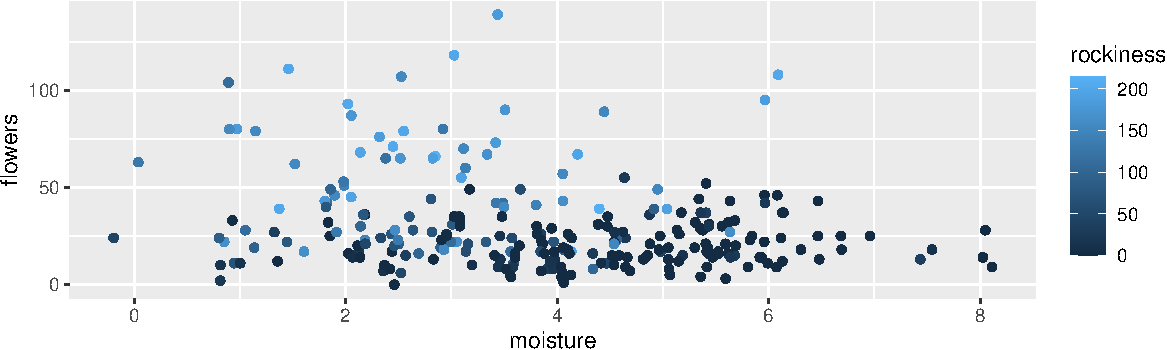
\includegraphics{Regression_and_ANOVA_files/figure-beamer/unnamed-chunk-10-1.pdf}

\end{frame}

\begin{frame}[fragile]{Interactions}
\protect\hypertarget{interactions}{}

To include an interaction term use \texttt{*} in the formula.
\scriptsize

\begin{Shaded}
\begin{Highlighting}[]
\NormalTok{lm4 <-}\StringTok{ }\KeywordTok{lm}\NormalTok{(flowers}\OperatorTok{~}\NormalTok{vegetative}\OperatorTok{+}\NormalTok{gopher}\OperatorTok{+}\NormalTok{moisture}\OperatorTok{*}\NormalTok{rockiness, }\DataTypeTok{data=}\NormalTok{Lily_sum)}
\KeywordTok{summary}\NormalTok{(lm4)}\OperatorTok{$}\NormalTok{coefficients; }\KeywordTok{summary}\NormalTok{(lm4)}\OperatorTok{$}\NormalTok{adj.r.squared}
\end{Highlighting}
\end{Shaded}

\begin{verbatim}
##                       Estimate Std. Error   t value     Pr(>|t|)
## (Intercept)         4.51089921 4.36901681  1.032475 3.028476e-01
## vegetative          0.73337897 0.10491177  6.990435 2.484626e-11
## gopher             -1.07010284 0.38716595 -2.763938 6.135862e-03
## moisture            2.98270503 0.80817645  3.690661 2.745527e-04
## rockiness           0.24005485 0.03909441  6.140389 3.215459e-09
## moisture:rockiness -0.02271932 0.01035527 -2.193987 2.915712e-02
\end{verbatim}

\begin{verbatim}
## [1] 0.5782167
\end{verbatim}

\normalsize

The resulting model has a term for the product of the interacting
variables. \[
\widehat{\text{flw}}=4.51+0.73\text{veg}-1.07\text{gph}+2.98\text{mst}+0.24\text{rck}-0.02(\text{mst}\times\text{rck})
\] Or, alternatively \[
\widehat{\text{flw}}=4.51+0.73\text{veg}-1.07\text{gph}+(2.98-0.02\text{rck})\text{mst}+0.24\text{rck}
\]

\end{frame}

\begin{frame}{Categorical predictors}
\protect\hypertarget{categorical-predictors}{}

It is common for some or all of the predictor variables in a regression
to be categorical.

\begin{itemize}
\tightlist
\item
  Presence/ Absence
\item
  Treatment levels: (low, medium, high)
\item
  Species
\end{itemize}

Categorical variables are encoded for regression using \textbf{indicator
(dummy) variables}.

Example: \(X\) is a categorical variable with levels \(a\), \(b\),
\(c\). Arbitrarily choose \(a\) as the \textbf{reference level} and
define \[
Z_b=\begin{cases} 
0 & \mbox{if } X =a\text{ or }c \\
1 & \mbox{if } X=b 
\end{cases}
\qquad
Z_c=\begin{cases} 
0 & \mbox{if } X = a \text{ or } b\\
1 & \mbox{if } X=c 
\end{cases}
\]

\end{frame}

\begin{frame}{One way ANOVA}
\protect\hypertarget{one-way-anova}{}

Continuing with the above example. Given data, regression will estimate
the parameters for a model \[
Y \sim N(\beta_0+\beta_1Z_b+\beta_2Z_c, \sigma^2).
\]

\begin{itemize}
\tightlist
\item
  If \(X=a\), the model predicts \(\hat y= \hat\beta_0\).
\item
  If \(X=b\), the model predicts \(\hat y= \hat\beta_0 + \hat\beta_1\).
\item
  If \(X=c\), the model predicts \(\hat y= \hat\beta_0 + \hat\beta_2\).
\end{itemize}

The hypothesis test using the \(F\) statistic as above to test \[
H_0: \beta_1=\beta_2=0, \quad H_a: \text{At least one of $\beta_1$ or $\beta_2$ is non-zero}
\] is what is classically called \textbf{analysis of variance} or ANOVA.

\end{frame}

\begin{frame}[fragile]{Multi-way ANOVA}
\protect\hypertarget{multi-way-anova}{}

Regression with multilple categorical predictors is called
\textbf{multi-way} or \textbf{multi-factor anova}.

\href{https://sakai.unc.edu/access/content/group/3d1eb92e-7848-4f55-90c3-7c72a54e7e43/public/docs/lectures/lecture2.htm\#description}{Tadpole
data} acquired from Weiss (2012). Note unequal variances. \scriptsize

\begin{Shaded}
\begin{Highlighting}[]
\NormalTok{tadpoles <-}\StringTok{ }\KeywordTok{read.csv}\NormalTok{(}\StringTok{"data/tadpoles.csv"}\NormalTok{)}
\NormalTok{tadpoles}\OperatorTok{$}\NormalTok{fac3 <-}\StringTok{ }\KeywordTok{as.factor}\NormalTok{(tadpoles}\OperatorTok{$}\NormalTok{fac3) }\CommentTok{# It's coded as 1 or 2.}
\KeywordTok{ggplot}\NormalTok{(tadpoles, }\KeywordTok{aes}\NormalTok{(fac3, response, }\DataTypeTok{fill =}\NormalTok{ fac2))}\OperatorTok{+}
\StringTok{  }\KeywordTok{geom_boxplot}\NormalTok{()}\OperatorTok{+}\KeywordTok{facet_wrap}\NormalTok{(}\OperatorTok{~}\NormalTok{fac1)}\OperatorTok{+}
\StringTok{  }\KeywordTok{scale_fill_brewer}\NormalTok{(}\DataTypeTok{palette =} \StringTok{"Dark2"}\NormalTok{)    }\CommentTok{# The default colors get boring.}
\end{Highlighting}
\end{Shaded}

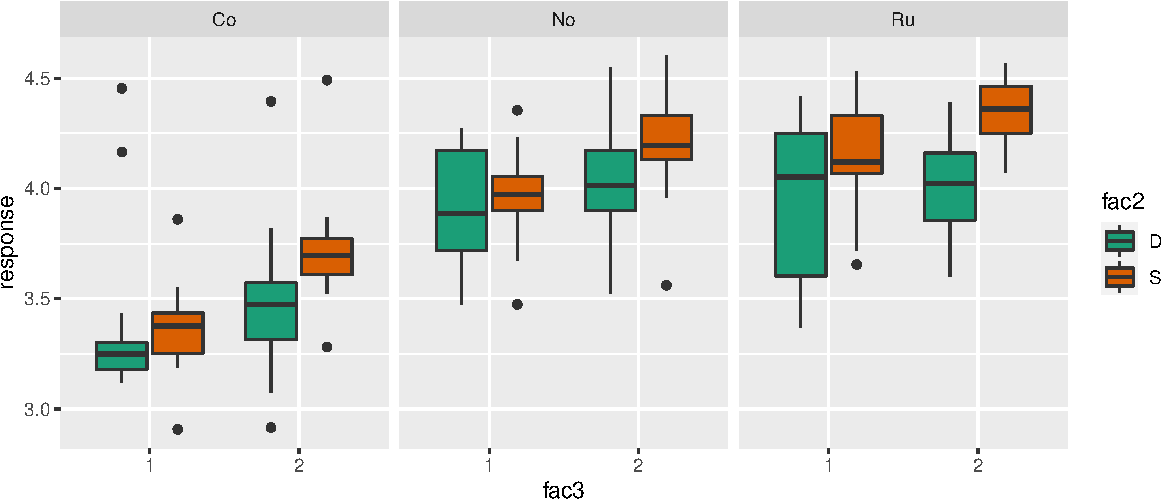
\includegraphics{Regression_and_ANOVA_files/figure-beamer/unnamed-chunk-12-1.pdf}

\end{frame}

\begin{frame}{A more general \(F\) statistic}
\protect\hypertarget{a-more-general-f-statistic}{}

Earlier we used \(F\) to compare a model to the \textbf{null model},
with no predictors.

A more general \(F\) statistic can compare any two models where one is
an extension of the other by adding predictors. To quantify the
advantage of a new model obtained by adding variables to an existing
model, compute \[
F = \frac{(SS_{old}-SS_{new})/(\text{number of new parameters} )}{SS_{new}/(\text{number of data points less parameters})}.
\]

\begin{itemize}
\tightlist
\item
  The number of new parameters, called the \textbf{numerator degrees of
  freedom} is the count of additional indicator variables in the
  extended model.
\item
  The \textbf{denominator degrees of freedom} is the number of data
  points minus the total number of parameters in the extended model.
\end{itemize}

\end{frame}

\begin{frame}[fragile]{ANOVA tables}
\protect\hypertarget{anova-tables}{}

The \texttt{anova} command calculates \(F\) statistics to compare
models.

\scriptsize

\begin{Shaded}
\begin{Highlighting}[]
\NormalTok{lm5 <-}\StringTok{ }\KeywordTok{lm}\NormalTok{(response}\OperatorTok{~}\NormalTok{fac1}\OperatorTok{*}\NormalTok{fac2}\OperatorTok{*}\NormalTok{fac3, }\DataTypeTok{data =}\NormalTok{ tadpoles)}
\KeywordTok{anova}\NormalTok{(lm5) }\CommentTok{# summary is not as useful as it analyzes indicator variables}
\end{Highlighting}
\end{Shaded}

\begin{verbatim}
## Analysis of Variance Table
## 
## Response: response
##                 Df  Sum Sq Mean Sq  F value    Pr(>F)    
## fac1             2 18.4339  9.2169 151.7899 < 2.2e-16 ***
## fac2             1  1.5013  1.5013  24.7238 1.304e-06 ***
## fac3             1  2.2771  2.2771  37.5007 3.984e-09 ***
## fac1:fac2        2  0.3926  0.1963   3.2328   0.04127 *  
## fac1:fac3        2  0.0838  0.0419   0.6900   0.50263    
## fac2:fac3        1  0.3503  0.3503   5.7693   0.01711 *  
## fac1:fac2:fac3   2  0.0695  0.0347   0.5723   0.56505    
## Residuals      227 13.7838  0.0607                       
## ---
## Signif. codes:  0 '***' 0.001 '**' 0.01 '*' 0.05 '.' 0.1 ' ' 1
\end{verbatim}

\normalsize

It appears that \texttt{fac1}, \texttt{fac2} and \texttt{fac3} all have
significant effects on the response, as do the interactions
\texttt{fac1:fac2} and \texttt{fac2:fac3}.

\end{frame}

\begin{frame}[fragile]{The model suggested by the ANOVA}
\protect\hypertarget{the-model-suggested-by-the-anova}{}

Now we can build a model using only those terms listed as significant.
\scriptsize

\begin{Shaded}
\begin{Highlighting}[]
\NormalTok{lm5a <-}\StringTok{ }\KeywordTok{lm}\NormalTok{(response}\OperatorTok{~}\NormalTok{fac1}\OperatorTok{+}\NormalTok{fac2}\OperatorTok{+}\NormalTok{fac3}\OperatorTok{+}\NormalTok{fac1}\OperatorTok{:}\NormalTok{fac2}\OperatorTok{+}\NormalTok{fac2}\OperatorTok{:}\NormalTok{fac3, }\DataTypeTok{data =}\NormalTok{ tadpoles)}
\KeywordTok{summary}\NormalTok{(lm5a)}\OperatorTok{$}\NormalTok{coefficients}
\end{Highlighting}
\end{Shaded}

\begin{verbatim}
##                Estimate Std. Error    t value      Pr(>|t|)
## (Intercept)  3.38323831 0.05245374 64.4994720 1.024057e-149
## fac1No       0.54729873 0.05837246  9.3759750  6.582616e-18
## fac1Ru       0.53698650 0.06084917  8.8248782  2.755469e-16
## fac2S        0.01714866 0.06696214  0.2560949  7.981054e-01
## fac32        0.10757945 0.04814860  2.2343214  2.641948e-02
## fac1No:fac2S 0.01341375 0.07727544  0.1735836  8.623448e-01
## fac1Ru:fac2S 0.16350360 0.08174704  2.0001164  4.665860e-02
## fac2S:fac32  0.16322994 0.06504617  2.5094473  1.277781e-02
\end{verbatim}

\normalsize

Note that the coefficients on \texttt{fac2S} and \texttt{fac1No:fac2S}
are not significant, it is only in its interactions with \texttt{fac1Ru}
and \texttt{fac32} that the diet factor appears to have an effect. We
will still include these terms in the model, because if we include an
interaction effect, we also include the corresponding main effects, and
if we include an effect from one level of a factor, we include all
levels.

\end{frame}

\begin{frame}[fragile]{Interpreting the result}
\protect\hypertarget{interpreting-the-result}{}

Plot the coefficients with confidence intervals. \tiny

\begin{Shaded}
\begin{Highlighting}[]
\NormalTok{ests <-}\StringTok{ }\KeywordTok{coef}\NormalTok{(lm5a)[}\OperatorTok{-}\DecValTok{1}\NormalTok{] }\CommentTok{# The reference level is not of immediate interest.  }
\NormalTok{tad_model <-}\StringTok{ }\KeywordTok{data.frame}\NormalTok{(}\DataTypeTok{var.labels=}\KeywordTok{factor}\NormalTok{(}\KeywordTok{names}\NormalTok{(ests), }\DataTypeTok{levels=}\KeywordTok{names}\NormalTok{(ests)), ests, }
                        \DataTypeTok{low95 =} \KeywordTok{confint}\NormalTok{(lm5a)[}\OperatorTok{-}\DecValTok{1}\NormalTok{,}\DecValTok{1}\NormalTok{], }\DataTypeTok{up95 =} \KeywordTok{confint}\NormalTok{(lm5a)[}\OperatorTok{-}\DecValTok{1}\NormalTok{,}\DecValTok{2}\NormalTok{])}
\KeywordTok{ggplot}\NormalTok{(tad_model, }\KeywordTok{aes}\NormalTok{(var.labels, ests))}\OperatorTok{+}
\StringTok{  }\KeywordTok{geom_pointrange}\NormalTok{(}\KeywordTok{aes}\NormalTok{(}\DataTypeTok{ymin=}\NormalTok{low95, }\DataTypeTok{ymax=}\NormalTok{up95))}\OperatorTok{+}
\StringTok{  }\KeywordTok{geom_hline}\NormalTok{(}\DataTypeTok{yintercept=}\DecValTok{0}\NormalTok{, }\DataTypeTok{linetype =} \StringTok{"dashed"}\NormalTok{, }\DataTypeTok{color =} \StringTok{"red"}\NormalTok{)}\OperatorTok{+}
\StringTok{  }\KeywordTok{labs}\NormalTok{(}\DataTypeTok{x =} \StringTok{"Term"}\NormalTok{, }\DataTypeTok{y =}  \StringTok{"Effect"}\NormalTok{)}\OperatorTok{+}\StringTok{ }\KeywordTok{coord_flip}\NormalTok{()}
\end{Highlighting}
\end{Shaded}

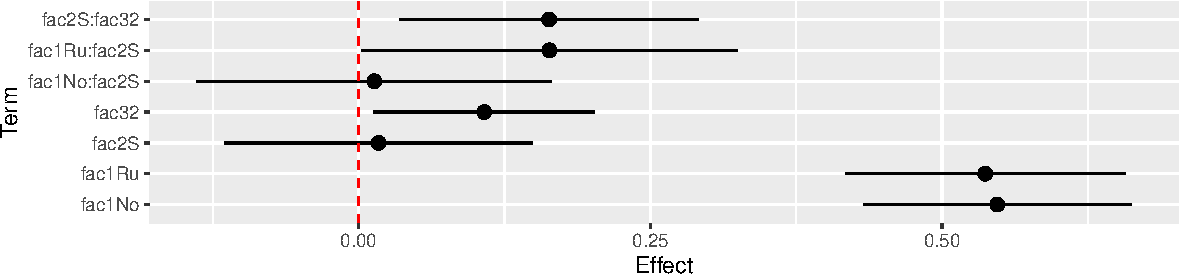
\includegraphics{Regression_and_ANOVA_files/figure-beamer/unnamed-chunk-15-1.pdf}
\normalsize The reference treatment is \texttt{CoD1}.

\begin{itemize}
\tightlist
\item
  \texttt{Ru} and \texttt{No} differ from \texttt{Co} but not each
  other.
\item
  On its own, Diet does not have a significant effect.
\item
  Sibships 1 and 2 have different mitotic levels.
\item
  Shrimp in combination with \texttt{Ru} or sibship 2 has an effect.
\end{itemize}

\end{frame}

\begin{frame}[fragile]{Type I (Sequential) and Type II (Marginal) ANOVA}
\protect\hypertarget{type-i-sequential-and-type-ii-marginal-anova}{}

\textbf{Type I} anova \textbf{sequential}ly adds each term in a list to
a model containing the terms before it on that list.

\textbf{Type II} or \textbf{marginal} anova compares a model to the
model including all possible other terms.

Often, type II is preferred. For example, why evaluate \texttt{fac1}
against the null model, \texttt{fac2} against \texttt{fac1}, and
\texttt{fac3} against \texttt{fac1} and \texttt{fac2} if the order in
which they are labelled is arbitrary?

Additionally, type II anova is more robust to deviations from the
assumption of equal group sizes, resulting in unbalanced designs.

\end{frame}

\begin{frame}[fragile]{Marginal ANOVA using the \texttt{car} package}
\protect\hypertarget{marginal-anova-using-the-car-package}{}

The base R command \texttt{anova} does sequential anova. Marginal anova
is done using the \texttt{Anova} command in the \texttt{car} package.

\scriptsize

\begin{Shaded}
\begin{Highlighting}[]
\KeywordTok{Anova}\NormalTok{(lm5)}
\end{Highlighting}
\end{Shaded}

\begin{verbatim}
## Anova Table (Type II tests)
## 
## Response: response
##                 Sum Sq  Df  F value    Pr(>F)    
## fac1           18.0783   2 148.8618 < 2.2e-16 ***
## fac2            1.6498   1  27.1702 4.184e-07 ***
## fac3            2.2300   1  36.7243 5.609e-09 ***
## fac1:fac2       0.2997   2   2.4681   0.08702 .  
## fac1:fac3       0.0550   2   0.4525   0.63659    
## fac2:fac3       0.3503   1   5.7693   0.01711 *  
## fac1:fac2:fac3  0.0695   2   0.5723   0.56505    
## Residuals      13.7838 227                       
## ---
## Signif. codes:  0 '***' 0.001 '**' 0.01 '*' 0.05 '.' 0.1 ' ' 1
\end{verbatim}

\normalsize

Results are similar to the type I analysis, but the p values for
\texttt{fac1:fac2} are on opposite sides of the bright line of \(0.05\).

\end{frame}

\begin{frame}[fragile]{Combining numerical and categorical predictors}
\protect\hypertarget{combining-numerical-and-categorical-predictors}{}

Often we have both numerical and categorical predictors.

Seed production example from Crawley (2012, 538).

\scriptsize

\begin{Shaded}
\begin{Highlighting}[]
\NormalTok{ipo <-}\StringTok{ }\KeywordTok{read.csv}\NormalTok{(}\StringTok{'data/ipomopsis.csv'}\NormalTok{)}
\KeywordTok{ggplot}\NormalTok{(}\DataTypeTok{data=}\NormalTok{ipo, }\KeywordTok{aes}\NormalTok{(}\DataTypeTok{x=}\NormalTok{Root, }\DataTypeTok{y=}\NormalTok{Fruit, }\DataTypeTok{color =}\NormalTok{ Grazing))}\OperatorTok{+}
\StringTok{  }\KeywordTok{geom_point}\NormalTok{()}
\end{Highlighting}
\end{Shaded}

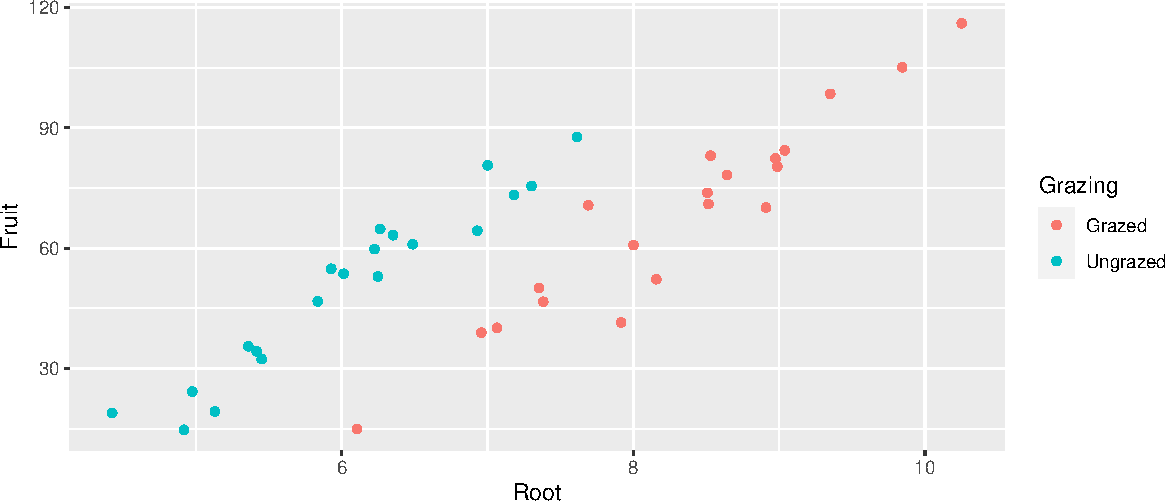
\includegraphics{Regression_and_ANOVA_files/figure-beamer/unnamed-chunk-17-1.pdf}

\end{frame}

\begin{frame}[fragile]{ANCOVA}
\protect\hypertarget{ancova}{}

Does the categorical predictor \texttt{Grazing} effect the numerical
response \texttt{Fruit}? The numerical variable \texttt{Root} is a
confounder. This is classical \textbf{analysis of covariance} or ANCOVA.
Once again, it's just regression.

\scriptsize

\begin{Shaded}
\begin{Highlighting}[]
\NormalTok{lm6<-}\StringTok{ }\KeywordTok{lm}\NormalTok{(Fruit}\OperatorTok{~}\NormalTok{Root}\OperatorTok{*}\NormalTok{Grazing, }\DataTypeTok{data=}\NormalTok{ipo)}
\KeywordTok{anova}\NormalTok{(lm6) }\CommentTok{# sequential and marginal are identical in this case}
\end{Highlighting}
\end{Shaded}

\begin{verbatim}
## Analysis of Variance Table
## 
## Response: Fruit
##              Df  Sum Sq Mean Sq  F value    Pr(>F)    
## Root          1 16795.0 16795.0 359.9681 < 2.2e-16 ***
## Grazing       1  5264.4  5264.4 112.8316 1.209e-12 ***
## Root:Grazing  1     4.8     4.8   0.1031      0.75    
## Residuals    36  1679.6    46.7                       
## ---
## Signif. codes:  0 '***' 0.001 '**' 0.01 '*' 0.05 '.' 0.1 ' ' 1
\end{verbatim}

\normalsize

\begin{itemize}
\tightlist
\item
  \texttt{Root} and \texttt{Fruit} appear correlated.
\item
  \texttt{Grazing} and \texttt{Fruit} appear correlated.
\item
  The interaction between \texttt{Grazing} and \texttt{Root} does not
  appear to affect \texttt{Fruit}.
\end{itemize}

\end{frame}

\begin{frame}[fragile]{Homogeneity of Variance}
\protect\hypertarget{homogeneity-of-variance}{}

Regression assumes that the variance in the residuals is constant for
all values of the predictors, or \textbf{homoscedasticity}. For real
data, we must asses the variance in the residuals against each
predictor.

In the tadpole data, the \texttt{CoD1}, \texttt{CoD2} and \texttt{RuD1}
treatment groups have higher variances than the others. Is this a
problem? \scriptsize

\begin{Shaded}
\begin{Highlighting}[]
\KeywordTok{ggplot}\NormalTok{(tadpoles, }\KeywordTok{aes}\NormalTok{(treatment, response))}\OperatorTok{+}
\StringTok{  }\KeywordTok{stat_summary}\NormalTok{(}\DataTypeTok{fun=}\NormalTok{var, }\DataTypeTok{geom=}\StringTok{"point"}\NormalTok{, }\DataTypeTok{shape =} \DecValTok{23}\NormalTok{) }\CommentTok{# Show variances.}
\end{Highlighting}
\end{Shaded}

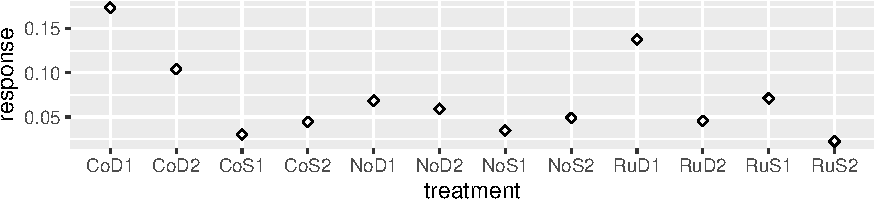
\includegraphics{Regression_and_ANOVA_files/figure-beamer/unnamed-chunk-19-1.pdf}
\normalsize

\begin{itemize}
\tightlist
\item
  For the \texttt{CoD1} and \texttt{CoD2} groups, the variance is due to
  outliers. Run the analysis without them - does the result change?
\item
  \texttt{RuD1} might be a problem, but it is only one group, and while
  the variance is large, at least there isn't much skew.
\end{itemize}

\end{frame}

\begin{frame}{Independence of observations}
\protect\hypertarget{independence-of-observations}{}

Regression assumes that observations are independent, but this is often
violated for real data.

\textbf{Pseudoreplication} is the technical term for data that includes
dependent observations. It has the effect of artificially increasing the
power of statistical tests. There are two very common scenarios where it
is encountered:

\begin{itemize}
\tightlist
\item
  \textbf{Repeated measures}: Observe the same individual multiple
  times.
\item
  \textbf{Block designs} and \textbf{Split plots}: Values of one
  variable are constant for grouped sets of observations.
\end{itemize}

We will discuss solutions to these issues later in the course.

\end{frame}

\begin{frame}{References}
\protect\hypertarget{references}{}

\hypertarget{refs}{}
\leavevmode\hypertarget{ref-crawley}{}%
Crawley, Michael J. 2012. \emph{The R Book}. 2nd ed. Wiley Publishing.

\leavevmode\hypertarget{ref-lily}{}%
Thomson, James D., George Weiblen, Barbara A. Thomson, Satie Alfaro, and
Pierre Legendre. 1996. ``Untangling Multiple Factors in Spatial
Distributions: Lilies, Gophers, and Rocks.'' \emph{Ecology} 77 (6):
1698--1715. \url{http://www.jstor.org/stable/2265776}.

\leavevmode\hypertarget{ref-weiss}{}%
Weiss, Jack. 2012. ``Ecology 563.''

\end{frame}

\end{document}
